\problemname{Pariserhjulet}
\illustration{0.3}{image}{Singapore Flyer \newline © CEphoto, Uwe Aranas}%
%
Efter att ha följt en mycket väloptimerad rutt genom flygplatsen är det svenska laget äntligen framme vid IOI i Singapore.
Under den första exkursionen får alla $N$ lag på IOI åka i det jättestora pariserhjulet Singapore Flyer.
Pariserhjulet har $M$ stycken vagnar och det tar även $M$ minuter för hjulet att snurra ett varv
(det tar alltså 1 minut för varje vagn att flyttas ett steg).

Vissa lag verkar vara mer intresserade av att åka pariserhjul än andra, och därför får varje lag bestämma exakt hur många varv de vill åka.
Det blir tråkigt för deltagarna om de måste gå av och sedan på igen innan de har åkt alla sina varv.
Det har därför bestämts att när ett lag väl har satt sig i en vagn, så får detta lag sitta kvar i vagnen fram till att de har åkt alla sina varv.
Detta betyder att om hjulet snurrar så att en vagn kommer ner till ingången, men det redan sitter ett lag i vagnen som vill fortsätta åka,
så kan nästa lag inte gå in i vagnen. Detta lag måste då vänta på en tom vagn eller en vagn med ett lag som går av.

Lagen är väldigt effektiva på att gå in och ut ur vagnarna, så det tar ingen extra tid att byta lag i den nedersta vagnen.

Alla lag står just nu i kö framför pariserhjulet, och det svenska laget undrar hur lång tid det kommer ta innan alla har åkt.

\section*{Indata}
Den första raden innehåller heltalen $N$ och $M$ separerade med blanksteg,
antalet lag och antalet vagnar i pariserhjulet.
Den andra raden innehåller $N$ heltal $T_1 ... T_N$ separerade med blanksteg,
där $T_i$ är antalet varv lag nummer $i$ vill åka. Lagen är ordnade efter
köplats, där $T_1$ är det första laget i kön.

\section*{Utdata}
Skriv ut en rad med ett heltal, antalet minuter det kommer ta för alla lag att åka.

\section*{Begränsningar}
Din lösning kommer att testas på en uppsättning testgrupper, var och en värd en viss poäng.
Varje testgrupp innehåller flera testfall.
För att få poäng för en testgrupp måste du klara alla testfallen i gruppen.
Din slutgiltiga poäng på problemet kommer att vara den maximala poängen av en enda inskickning.

\noindent
\begin{tabular}{| l | l | l |}
\hline
Grupp & Poäng & Gränser \\ \hline
1     & 20    & $1 \le N, M, T_i \le 100$ \\ \hline
2     & 30    & $1 \le N, M, T_i \le 1000$ \\ \hline
3     & 25    & $1 \le N, M \le 1000, 1 \le T_i \le 10^9$ \\ \hline
4     & 25    & $1 \le N, M \le 200\,000, 1 \le T_i \le 10^9$ \\ \hline
\end{tabular}

\section*{Förklaring av exempelfall}

\begin{figure}[h]
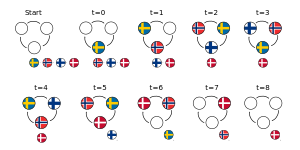
\includegraphics[width=0.8\textwidth]{sample1}
\caption{Exempelfall 1}
\end{figure}

I exempelfall 1 finns det 4 lag och 3 vagnar.
Lagen, som i bilden är Sverige, Norge, Finland och Danmark, vill åka 2, 2, 1 och 1 varv respektive.
Notera att det danska laget inte kan gå in i pariserhjulet vid $t=3$ eller $t=4$
eftersom det svenska / norska laget redan sitter i den nedersta vagnen och vill i båda fallen åka ett varv till.
